\section{Architektura IoT sítí}
  V blízké době se očekává stále větší nárůst zařízení, která jsou připojena k internetu.
  Dle odhadů by jejich počet měl v roce 2020 překročit 30 miliard \cite{iotDevices}.
  Pro takové množtví připojení už není možné, aby každé zařízení komunikovalo přímo
  se vzdáleným datovým centrem, protože nároky na potřebnou šířku pásma by byly 
  obrovské \cite{fog}.
  Dalším problémem je často velmi omezený výkon připojených prvků, který je nezbytný pro 
  použití bezpečnostních funkcí umožňujících kompletně zabezpezpečenou komunikaci. 
  
  Řešení těchto problémů je do probíhající komunikace přidat několik podvrstev, 
  které umožní přesunout výpočetní výkon blíže ke koncovým zařízením, a tím celý
  proces zpracování dat provést efektivněji.
 \subsection{Fog computing} 
 Fog computing je rozšíření Cloud computingu, které spočívá v přesunutí výpočetního
 výkonu blíže k okraji sítě. Rozšíření je umožněno pomocí přidání síťových zařízení,
 které kromě běžných funkcionalit poskytují i výpočetní výkon pro běh externích programů. Programy 
 je často možné nasadit pomocí kontejnerů nebo samostatných virtuálních strojů, což 
 velmi usnadňuje jejich distribuci \cite{fog}.
 
 Porovnání klasické a Fog architektury se nachází na obrázku \ref{obr.fog}. V reálném nasazení může
 být použito i více Fog vrstev, kde každá provádí určitý stupeň předzpracování a řízení
 dat.
\begin{figure}[ht]
\begin{center}
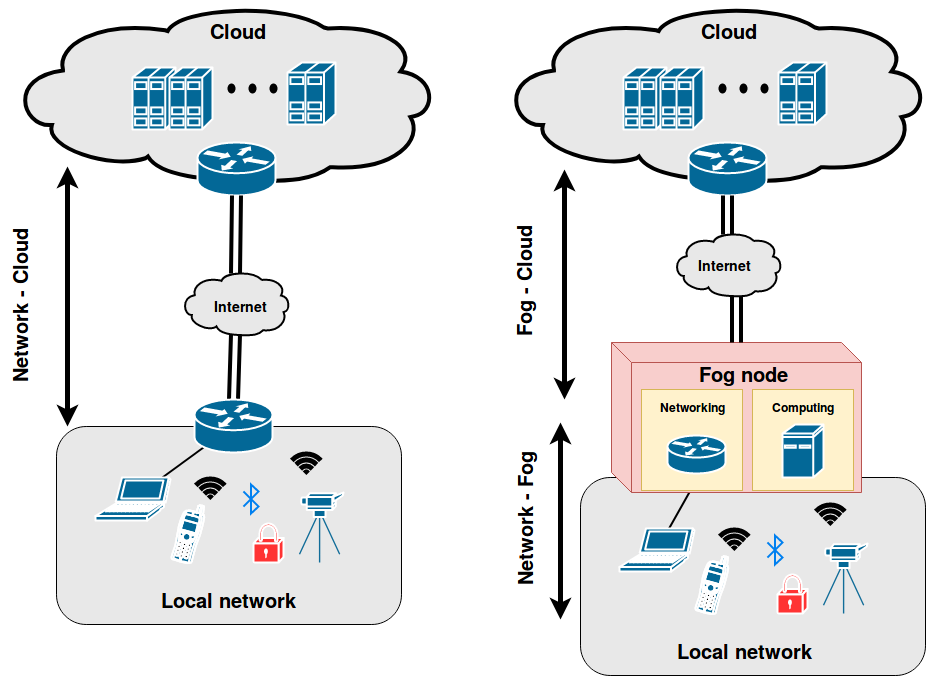
\includegraphics[scale=0.38]{pictures/fog}
\caption{Porovnání klasické a Fog architektury}
\label{obr.fog}
\end{center}
\end{figure}
 Zavedením principů Fog computingu vznikají pro síť následující výhody:
 \begin{itemize}
 \item \textbf{Zlepšení bezpečnosti} \cite{fog}
 
     Síťové prvky jsou trvale napájené a připojené k internetu. Podporují pokročilé
     bezpečnostní funkce, a proto je možné například vytvářet šifrované tunelové
     spojení pro bezpečný přenos dat.     
\item \textbf{Nižší nároky na šířku pásma a latency} \cite{fog}

    Odeslaná data z koncových zařízení jsou zpracovávána a filtrována na okraji 
    sítě. Tím je možné rychleji reagovat na přijaté zprávy a snížit nároky
    na latency a šířku pásma. Zároveň krátkodobá data mohou být uložené ve 
    Fog vrstvě a centrální datové cetrum může být využito pro dlouhodobé údaje, 
    které se zpracovávají pokročilými algoritmy pro analýzu dat.
 \item \textbf{Jednotná správa} \cite{fog}
 
    Při správě sítě už se nemusí přistupovat přímo na koncové prvky, které 
    často komunikují různými protokoly, ale stačí pouze
    řídit síťová zařízení v jednotlivých Fog vrstvách, které odstiňují různorodost
    protokolů a nabízí standardizovaný přístup. Díky této abstrakci je 
    zároveň zjednodušeno zpracování získaných dat a je umožněno přímé zasílání zpráv
    mezi koncovými prvky, které používají odlišné komunikační protokoly.
 \end{itemize} 
 
 \subsection{IoT brána} 
 IoT brána je síťové zařízení, které je umístěno velmi blízko koncových zařízení
 a představuje vstup do Fog vrstvy. Jejím hlavním cílem je získávat data 
 z připojených zařízení a poskytovat je vyšším vrstvám. Pokud je brána reprezentována
 výkonnějším síťovým prvkem, tak v rámci brány může probíhat i základní zpracování
 dat. 
 
 Pro IoT sítě je typické, že obsahují velké množtví koncových prvků komunikujících
 různorodými způsoby. Zejména senzory použivají protokoly, které nepodporují
 IP spojení. Důvodem použití této komunikace je často velký
 důraz na nízkou spotřebu a specifické požadavky na způsob zasílání zpráv.
 Příkladem protokolů pro senzorové sítě je například:
 Z-Wave, Bluetooth a Zigbee. Jejich detailní popis se nachází v kapitole \ref{protokoly}.
 Tato různorodost vyžaduje, aby brána obsahovala dodatečná rozhranní, které 
 umožní připojení nejrůznějších bezdrátových i drátových koncových prvků. 
 
 V součastné době existuje mnoho různých bran jejichž parametry se liší dle 
 způsobu nasazení a provozních nároků. Velkým problémem v této oblasti je malý 
 důraz na bezpečnostní funkce, které umožní vzdálené řízení brány, kontrolu provozu a 
 aktualizace programového vybavení. Z těchto důvodů vznikl opensource projekt BeeeOn \cite{beeeon}
 jehož cílem je vytvořit softwarou IoT bránu, kterou bude možné spustit na různých 
 hardwarových platformách. BeeeOn brána je navržena modulárně tak, aby byla schopna 
 zpracovávat více rozdílných senzorových protokolů, a tím je možné provozovat jedno
 univerzální zařízení namísto několika proprietárních. Zároveň je kladen důraz na bezpečnost 
 a veškeré údaje, které je možné získat o provozu, jsou poskytovány pro analýzu. Nad těmito údaji
 je postaven detekční algoritmus, který je výsledkem této diplomové práce.
 
 %přidat popis BeeeOn

 \subsection{Komunikační model a jeho hrozby}
 Při použití principů popsaných v předchzích kapitolách lze model komunikace
 do následujících vrstev \cite{iotSurvey}:
 \begin{itemize}
 \item Aplikační vrstva 
 \item Síťová vrstva
 \item Senzorová vrstva
\end{itemize}
 Jednotlivé vrstvy budou popsány v následujích podkapitolách.
 
 \subsubsection{Senzorová vrstva}
 Senzorová vrstva obsahuje veškerá koncová zařízení, které získávají informace ze svého
 okolí nebo vykonávají potřebnou službu \cite{secFramework}. Tato zařízení jsou připojena
 kabelově nebo bezdrátově k IoT bráně. K jedné bráně může být připojeno několik
 prvků, které komunikují odlišnými způsoby.
 
 Velkým nebezpečím této vrstvy jsou zejména bezdrátové protokoly, protože při nepoužití
 zabezpečení může snadno dojít k odposlouchávání nebo úprávám provozu \cite{iotSurvey}.
 Dále se zde mohou vyskytovat zařízení, které jsou označeny jako zabezpečené, 
 ale používají zastaralé bezpečnostní funkce nebo obsahují implementační chyby. 
 Tento případ je velmi nebezpeční, protože vyvolává falešný pocit bezpečí.
 
 \subsubsection{Síťová vrstva}
 Po zpracování senzorových dat na bráně je nutné získané informace odeslat dalším
 službám. K tomuto účelu slouží síťová vrstva. Cílem této vrstvy je také umožnění 
 vzdálené správy brány \cite{secFramework}. Pro výběr konkrétního protokolu je 
 nutné znát rozhranní aplikační vrstvy. Nicméně spojení je většinou vytvořeno
 pomocí protokolu HTTPS (Hypertext Transfer Protocol Secure) nebo technologie
 VPN (Virtual Private Network). Nad tímto spojením je postaven další služba pro 
 výměnu zpráv. Příkladem může být: MQTT (Message Queuing Telemetry Transport),
 COAP (Constrained Application Protocol),
 AMQP (Advanced Message Queuing Protocol).
 
 Bezpečnostní hrozby této vrstvy jsou stejné jako v klasických sítích. Je potřeba
 dodržet principy důvěry, integrity a dostupnosti. Tímto přístupem je možné
 předejít útokům jako: DDoS (Distributed Denial Of Service),
 MITM (Man In The Middle) a podvržení informací. Zároveň je nutné
 nezapomenout, že se zde většinou vyskytuje M2M (Machine To Machine)
 komunikace a je důležité použít 
 vhodná komunikační rozhranní \cite{iotSurvey}.
 
 \subsubsection{Aplikační vrstva}
 Aplikační vrstva se stará o ukládání dlouhodobých dat a jejich finální zpracování. 
 Zároveň zobrazuje uživateli zpracované informace a umožňuje provádět konfiguraci
 celé sítě. Z důvodu možné rozsáhlosti celé sítě je kritické, aby správa
 topologie podporovala automatizaci. \cite{secFramework}.
 
 Tato vrstva je umístěna vetšinou v datovém centru a umožňuje vzdálený přístup. 
 Její bezpečnostní problémy lze přirovnat k problémům cloud computingu. Dle
 množtví požadovaných funkcí může být různě složitá a s rostoucí složitostí
 se také liší nároky na úroveň zabezpečení. Příkladem možných útoků může být:
 Buffer Overflow, SQL Injection nebo DDoS.
 
 \section{Používané komunikační protokoly} \label{protokoly}
  \subsection{MQTT}
  \subsection{COAP}
 % popis funkce fungování MQTT, COAP, (AMQP)
 %\section{Analýza senzorových protokolů} \label{senzory}
  \subsection{Z-Wave}
  \subsection{Bluetooth}
 % popis a bezpečnostní analýza ZWave a Bluetooth
 \section{Bezpečnostní slabiny a možnosti detekce}
 \begin{itemize}
 \item Vnější vs vnitřní útoky
 \item Signature based vs Anomaly based
 \item paketová vs flow vs extended flow analýza
 \item Senzorová data - provozní data z driverů vs dedikované zařízení (SDR, ...)
\end{itemize}
 % popis IDS principů
 %vnitrni a vnejsi utoky
 %ziskavani statistickych dat ze senzorů
 %získávání statistickych dat z IP části

 \section{Existující řešení}
  \begin{itemize}
 \item Existuje řešení pomocí Suricata, které používá Turris (centrální, signature
 based řešení)
 \item Neexistuje řešení, které by provádělo detekce z senzorových dat
 \item Neexistuje řešení, které by umožňovalo senzorové nebo pokročilé síťové
 detekce na bráně nebo mimo ni
\end{itemize}
 % aktuální řešení funguje na cetrálním monitorovacím prvku, které monitoruje IP
 % teprve nedávno vznikly signatury pro SCADA
 \section{Analýza požadavků}
 \section{Zvolené řešení}
